\chapter{醫學類}
\section{2016年2月1日 (Instructor: Vivian)}
\subsection{留學生抑鬱症}
\subsubsection*{需要掌握的單詞短語}
\begin{multicols}{2}
\begin{itemize}
  \itemsep0em
  \item 力氣: energy / strength
  \item 養活: support life
  \item 另一個自己: another me / self
  \item 離婚: divorce (及物動詞) divorce sb. (表示離婚的動作)
  \item 同父異母, 同母異父的兄弟: half brother
  \item 導致的原因: contributing factor
  \item 跟蹤: stalk / stalking
  \item 真理 / 真實存在的: true / real
  \item 大傷口 / 一條一條的傷: wound / cut
  \item 自殺: suicide (注意是名詞), 表示自殺動作: commit suicide
  \item 積蓄: savings
  \item 割腕: cut my wrist / wrist cutting
  \item 跳樓: jump off \hilight{a} building
  \item 傷心到崩潰: be devastated
  \item 雙重人格 / 人格分裂: dual personality / split personality
\end{itemize}
\end{multicols}

\subsubsection*{需要掌握的句型}
\begin{multicols}{2}
\begin{itemize}
  \itemsep0em
  \item 建議某人做某事: sb. suggests \hilight{I} do sth. / asks \hilight{me} to do sth.
  \item 向MRT遞交投訴: lodge an appeal \hilight{with} MRT.
  \item 履行...義務: fulfill one's obligation.
  \item 不是不...而是...: It's not that... (接主動句), but it's because / it's just...
  \item 更詳細地解釋: explain...in more detail
  \item 忍不住做某事: I can't help / stop doing sth.
  \item 和某人結婚 / 離婚: get divorced / married with sb 或 get a divorce with ...
  \item 自從...就...: Since..., has / have been doing sth.
  \item 被診斷出: be diagnosed with...
  \item 離開去工作: left for work
  \item ``知道以後"的兩種說法
  \begin{enumerate}
    \itemsep0em
    \item after I know (強調我一直都知道)
    \item after I get to know / find out (強調從不知道到知道)
  \end{enumerate}
  \item 讓某人喘不過氣: suffocate sb.
  \item 發洩出來: let it out
  \item 負能量爆棚: full of negative energy
  \item 堅持做某事
  \begin{enumerate}
    \itemsep0em
    \item Insist on sth. / doing sth.
    \item Insist that + 從句 (e.g. sb. should do sth.)
  \end{enumerate}
  \item 恢復了正常的意識: came to someone's senses.
  \item 讓...過去吧: let go of sth.
  \item 好好學習: do well in my studies.
\end{itemize}
\end{multicols}

\subsection{助聽器}
\subsubsection*{需要掌握的單詞短語}
\begin{itemize}
  \itemsep0em
  \item 助聽器: hearing aid
  \item 聽力 / 視力矯正師: Audiologist / Optometrist
  \item 聽覺神經: auditory nerves
  \item 高檔的診所: \hilight{fancy}\footnote{fancy不一定非要指外觀花哨} clinic
\end{itemize}

\subsubsection*{需要掌握的句型}
\begin{itemize}
  \itemsep0em
  \item 直接告訴我: tell me \hilight{straight up} (後面無逗號接陳述句)
  \item 我看不清圖: I can't \hilight{read} the graph.
  \item 情況更嚴重了:
  \begin{enumerate}
    \itemsep0em
    \item Condition gets serious / worse
    \item Worsens / Deteriorates
  \end{enumerate}
  \item 正視困難: face up the problem
  \item 資助某人: fund sb.
\end{itemize}

\subsection{鼻炎 (共三部分)}
\subsubsection*{需要掌握的單詞短語}
\begin{multicols}{2}
\begin{itemize}
  \itemsep0em
  \item 過敏反應: allergy reaction
  \item 鼻竇炎 / 鼻炎: sinusitis (簡稱sinus) / rhinitis
  \item 過敏性 / 季節性鼻炎: allergic / seasonal rhinitis
  \item 小蟲咬的: insect bites
  \item 低燒: low grade fever
  \item \hilight{呼吸道: respiratory tract}
  \item 鼻塞: blocked / congested nose
  \item 十幾歲: in my \hilight{teens}
  \item 花粉 / 粉塵: pollen / dust
  \item 開花 / 花展: flowering / florae
  \item 異物: foreign material
  \item 威脅生命: life-threatening
  \item 呼吸道內壁: lining of the tract
  \item anaphylaxis = allergic reaction
  \item 營養不良: malnutrition
  \item 惡心: nauseous, nausea
  \item 化學氣味: chemical odour
  \item 乳糖: lactose
  \item 母乳: breastfeeding
  \item 流眼淚 / 鼻涕: streaming eyes (watery eyes) / nose
  \item 過敏源: allergens
\end{itemize}
\end{multicols}

\subsubsection*{需要掌握的句型}
\begin{multicols}{2}
\begin{itemize}
  \itemsep0em
  \item 她從來沒有得過(病): She has never had...
  \item 常見的小毛病:
  \begin{enumerate}
    \itemsep0em
    \item common ailment
    \item common minor illness
  \end{enumerate}
  \item 從...傳染的: got infected / caught / got it from...
  \item 引出...併發症: lead to / trigger / cause...
  \item 傳染性強的病毒性疾病: highly infected virus disease
  \item 不知什麼原因: for some reason
  \item 情況有所好轉: condition has improved / became batter.
  \item 我受夠他了: I am so fed up with sb.
\end{itemize}
\end{multicols}

\vspace{15mm}
\begin{center}
  \textbf{************ END OF THE DAY ************}
\end{center}
\newpage

\section{2016年2月2日 (Instructor: Chris)}
\subsection{肥胖症}
\subsubsection*{需要掌握的單詞短語}
\begin{multicols}{2}
\begin{itemize}
  \itemsep0em
  \item 避難所 / 安全島: refuge / refuge island
  \begin{center}
    
\includegraphics[scale=0.4]{pics/refuge-island}
  \end{center}
  \item 闖紅燈: run a red light (\hilight{run後面不加介詞})
  \begin{center}
    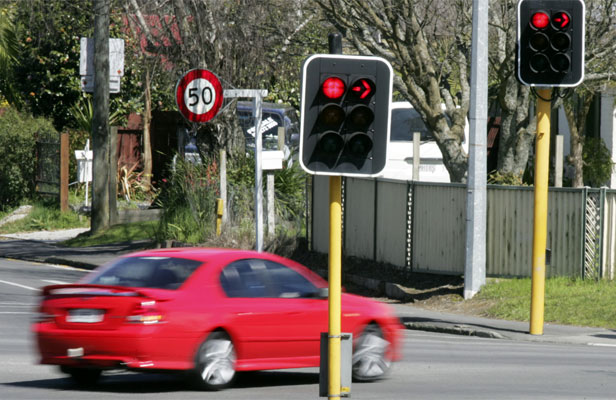
\includegraphics[scale=0.4]{pics/run-red-light}
  \end{center}
  \item 肥胖症: obesity ($n.$) / obese ($adj.$) 
  \item 心血管疾病: \hilight{cardiovascular} disease
  \item 體重指數: BMI (Body Mass Index)
  \begin{center}
    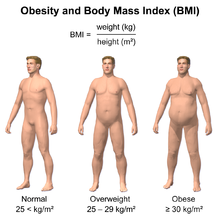
\includegraphics[scale=1]{pics/bmi}
  \end{center}
  \item 充血性心律衰竭: Congestive Heart \hilight{Failure} (failure在醫學里一般指\hilight{衰竭})
  \item 營養師: dietician / nutritionist
  \item 有氧運動: aerobics (一般30到40分鐘)
  \item 減肥藥: weight-loss pills
  \item 飲食配方: prescription diet
  \item 底線, ``關鍵是": bottom line
  \item 冥想: meditation
  \begin{center}
    
\includegraphics[scale=.3]{pics/meditation}
  \end{center}
  \item 規律: routine ($n.$ + $adj.$)
  \item energetic $\xrightarrow{\text{反義詞}}$ listless
  \item 暴食: binge eating
  \begin{center}
    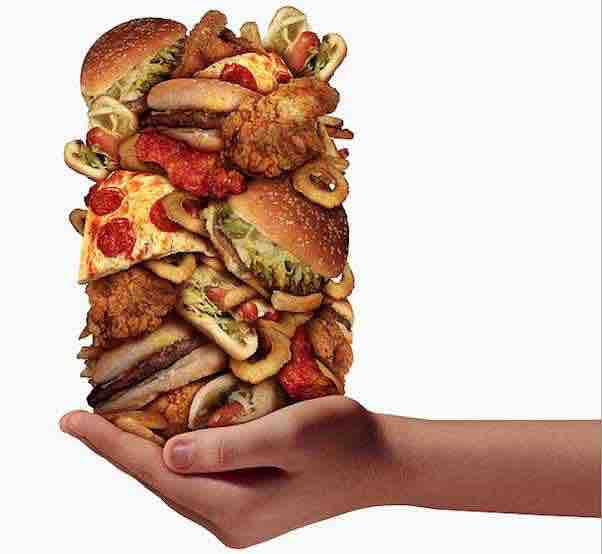
\includegraphics[scale=.3]{pics/binge-eating}
  \end{center}
  \item 碳水化合物: carbohydrate
\end{itemize}
\end{multicols}

\subsubsection*{需要掌握的句型}

\begin{itemize}
  \itemsep0em
  \item 少食多餐: eat more frequently but with less portion each meal.
  \item 我正想告訴你: I was going to tell you.
  \item 我稱了下體重: I \hilight{weighed} myself.
  \item stick to = keep doing...
  \item 量身定制...: It is tailored to...
  \item 試試: give / have a go / try
  \item 改善肥胖症:
  \begin{enumerate}
    \itemsep0em
    \item \hilight{improve} obesity
    \item recover from obesity
    \item treat obesity
  \end{enumerate}
  \item 與...一致/協調: in \hilight{tune} with...
  \item 往往: tend to...
\end{itemize}

\subsection{糖尿病}
\subsubsection*{需要掌握的單詞短語}
\begin{itemize}
  \itemsep0em
  \item 胰腺: pancreas $\xrightarrow{\text{分泌}}$ \hilight{insulin (胰島素)}
  \begin{center}
    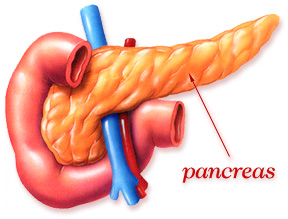
\includegraphics[scale=.5]{pics/pancreas}
  \end{center}
  \item 胰腺炎: pancreatitis
  \item impotence (陽痿) $\xrightarrow{\text{變成形容詞}}$ impotent \ \ \ \ \ \ \ \ frigidity (女性性冷淡) $\xrightarrow{\text{變成形容詞}}$ frigid
  \begin{center}
    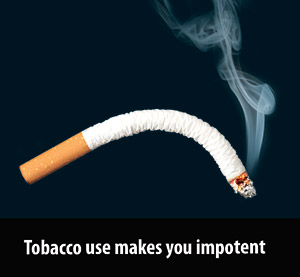
\includegraphics[scale=.6]{pics/impotence}
    
\includegraphics[scale=.45]{pics/frigidity}
  \end{center}
  \item 葡萄糖 / 甜食: glucose / sweets
  \begin{center}
    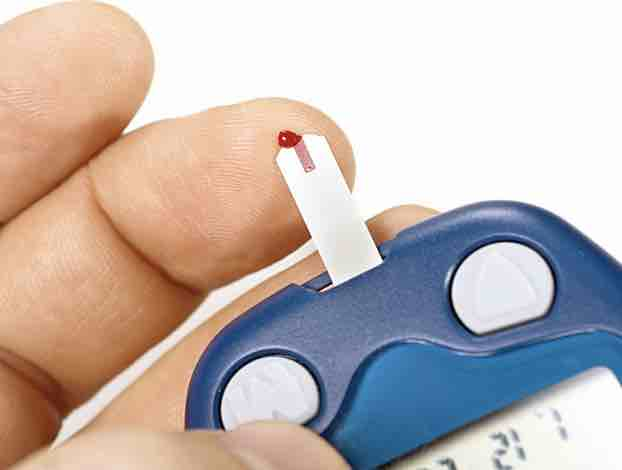
\includegraphics[scale=.2]{pics/glucose.jpg}
  \end{center}
  \item 內分泌科醫生: endocrinologist (endo代表內科, crino代表分泌)
  \item 截肢: amputation
  \item 飲食(表動作): dieting
  \item (血管中的)血流: bloodstream
\end{itemize}

\subsubsection*{需要掌握的句型}
\begin{itemize}
  \itemsep0em
  \item 喜食甜食者: have a sweet tooth \hilight{(tooth一定是單數)}.
  \item 堅持做某事: insist \hilight{on} doing sth / insist that + 從句.
  \item 您放心...: Let me reassure you...
  \item 我向您保證: Let me assure you...
  \item 徹底失明: lost someone's sight completely.
  \item 死於: \hilight{die of...(病) / die from...(天災人禍)}
  \item 非得這樣嗎?: Does it have to be the case?
\end{itemize}

\subsubsection*{其他}
\begin{itemize}
  \item 糖尿病的兩類:
  \begin{enumerate}
    \itemsep0em
    \item \textbf{Type I\footnote{1型糖尿病(舊稱青少年糖尿病或胰島素依賴型糖尿病)是糖尿病的一種類型,它與2型糖尿病的發病機理完全不同,\\屬於自體免疫性疾病,可能是基因或由於自體免疫系統破壞產生胰島素的胰腺胰島$\beta$細胞引起的,因此患者必須注射胰島素\\治療,目前世界上對此病沒有治癒方法。}} (genetic 先天的): insulin-dependent (胰島素依賴型)
    \item \textbf{Type II} (acquired 後天的): non-insulin dependent (非胰島素依賴型)
  \end{enumerate}
  \item 醫學里涉及的A, B, C, D在中文里要翻譯成\hilight{甲, 乙, 丙, 丁}.
  \item 廁所里看到的小箱子叫syringe disposal (註冊器丟棄), 一般用於insulin injection (胰島素注射).
  \begin{center}
    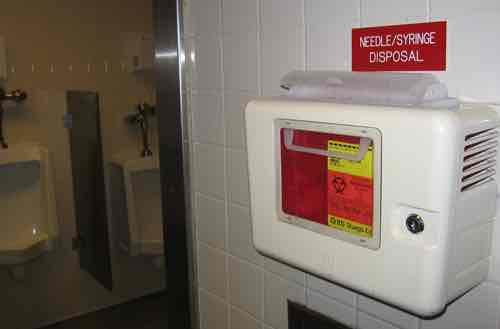
\includegraphics[scale=.6]{pics/syringe}
  \end{center}
\end{itemize}

\subsection{糖尿病檢查}
\mybox{\centering \textbf{注意}: 更多筆記被歸納到專題里的"人體的各種系統", 請參考目錄查找!}
\subsubsection*{需要掌握的單詞短語}
\begin{itemize}
  \itemsep0em
  \item (stress) echocardiogram: (負荷) 超聲波心動圖\footnote{超聲心動圖是應用超聲波回聲探查心臟和大血管以獲取有關信息的一組無創性檢查方法。包括M型超聲、二維超聲 、脈衝多普勒、連續多普勒、彩色多普勒血流顯像。}
  \item angiogram: 血管造影\footnote{血管造影是一種介入檢測方法,將顯影劑注入血管里,因為X光無法穿透顯影劑,血管造影正是利用這一特性,通過\\顯影劑在X光下所顯示的影像來診斷血管病變的。} (angio代表和血管有關)
  \begin{center}
    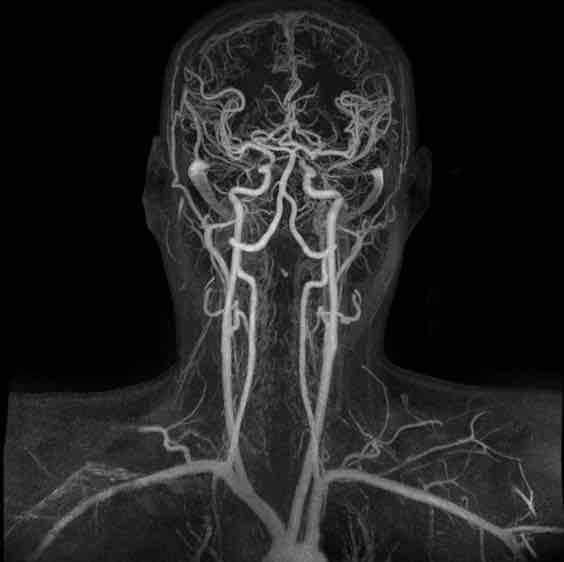
\includegraphics[scale=.3]{pics/angiogram}
  \end{center}
  \item 患妄想症的: paranoid $adj.$
  \item 惡化: deteriorate = get worse
  \item 劑量: dosage
  \item diabetes $\xrightarrow{\text{變成形容詞}}$ diabetic: $adj.$ 糖尿病的, $n.$ 糖尿病患者
  \item 癮: addiction
  \item 挫敗感: frustrated
  \item 人的三種血管: artery (動脈) / vein (靜脈) / capillary (毛細血管)
\end{itemize}

\subsection{針灸}
\subsubsection*{需要掌握的單詞短語}
\begin{itemize}
  \itemsep0em
  \item 針灸 / 針灸師: acupuncture / acupuncturist
  \item 手指:
  \begin{center}
    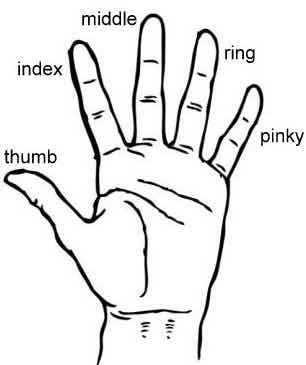
\includegraphics[scale=.55]{pics/fingers}
  \end{center}
  \item 穴位: acu-points
  \begin{center}
    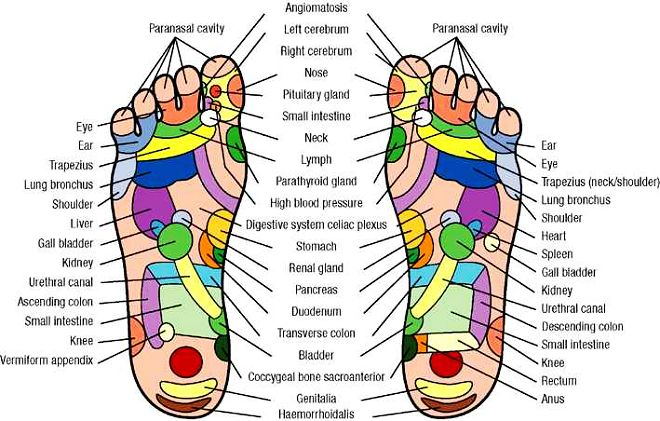
\includegraphics[scale=.75]{pics/acu-points}
  \end{center}
  \item 尼古丁貼劑: nicotine \hilight{patch} (patch還可以指膏藥)
  \begin{center}
    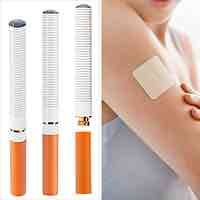
\includegraphics[scale=.7]{pics/nicotine-patches}
  \end{center}
  \item 有決心 / 有毅力: determined / \hilight{dedicated}
  \item 免疫力: immunity
  \item 一根煙 / 一包煙 / 一條煙: a cigarette a smoke / a \hilight{pack} of cigarettes / a \hilight{carton} of cigarettes
  \item 生理慾望: craving
  \item 大煙槍: chain / heavy smoker
  \item 鎮靜: sedate ($\sim$ $sb.$) / sedation (put $sb.$ under $\sim$)
  \item 鎮靜劑: sedative (依然是\hilight{$n.$}) \hilight{重音在前}
  \item 麻痹感: numb ($adj.$) $\xrightarrow{\text{變成名詞}}$ numbness
  \item 揉: rub
  \item 膠帶: tape
  \item 耳朵的: auricular
  \item 神經末梢: nerve ends
  \item 中樞神經系統: Central Nervous System
\end{itemize}

\subsubsection*{需要掌握的句型}
\begin{itemize}
  \itemsep0em
  \item 減少吸煙量: reduce amount of cigarette
  \item 每天少吸五根煙: smoke five cigarettes less per day
\end{itemize}

\subsection{飲食紊亂}
\subsubsection*{需要掌握的單詞短語}
\begin{itemize}
  \itemsep0em
  \item anorexia (厭食症) $\xrightarrow{\text{反義詞}}$ bulimia (暴食症)
  \item 青春期少女: adolescent girl
  \begin{center}
    
\includegraphics[scale=.4]{pics/adolescent}
  \end{center}
  \item 習慣做某事: \hilight{get} used to...
  \item 皮包骨: skinny
  \item 油脂的, 油膩的: greasy
  \begin{center}
    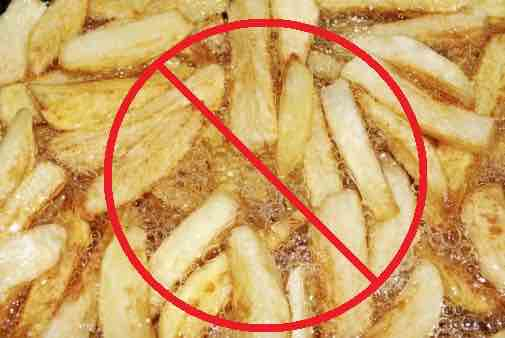
\includegraphics[scale=.5]{pics/greasy}
  \end{center}
  \item 反作用: \hilight{counter-productive}
  \item 兒童肥胖症: \hilight{childhood} obesity
\end{itemize}

\subsubsection*{需要掌握的句型}
\begin{itemize}
  \itemsep0em
  \item 少吃一頓飯: \hilight{skip} a meal
  \item 對...充耳不聞 / 視而不見: turn a deaf ear / blind eye to
  \item 體力活動變少: less physically active
  \item 讓某人明白: \hilight{get across to sb.} = make sb. understand
  \item 最好做: be better off doing sth.
\end{itemize}

\subsection{腸病}
\subsubsection*{需要掌握的單詞短語}
\begin{multicols}{2}
\begin{itemize}
  \itemsep0em
  \item 腹瀉: diarrhoea
  \item 腹痛: abdominal pain
  \item 腹脹: bloating
  \item 便秘: constipation
  \item 排便: bowel \textit{movement / motions / opening}
  \item 拉肚子: get the runs
  \item 不舒服: discomfort (不是un做前綴)
  \item colonoscopy: (結)腸鏡 (scopy代表醫用內窺鏡)
  \item 腸道易激綜合症: Irritable Bowel Syndrome\footnote{腸易激綜合徵(IBS)是一組持續或間歇發作,以腹痛、腹脹、排便習慣和(或)大便性狀改變為臨床表現,而缺乏胃\\腸道結構和生化異常的腸道功能紊亂性疾病。典型症狀為與排便異常相關的腹痛、腹脹,根據主要症狀分為:腹瀉主導型;\\便秘主導型;腹瀉便秘交替型。精神、飲食、寒冷等因素可誘使症狀復發或加重。}
  \item 非典型的: atypical
  \item 嚴重急性呼吸綜合症: Severe Acute Respiratory Syndrome (SARS) \footnote{是非典型肺炎的一種。中國簡稱為非典,根據英文發音有沙士、薩斯病、沙斯病或煞斯病等多種譯名。}
  \item 息肉 (ployp) $\xrightarrow{\text{惡性}}$ bowel cancer $\xrightarrow{\text{結腸}}$ colon cancer
  \item 輪流出現: alternative = take turns
  \item 篩查測試: \hilight{screening} test
  \item 化驗科, 病理學實驗室: pathology lab
  \item 排泄物潛隱血檢查: Fecal Occult Blood Test (FOBT) \footnote{糞便潛隱血(FOB)是指糞便中帶隱形血。糞便潛隱血測試通過將糞便塗抹於測試條進行檢查。}
\end{itemize}
\end{multicols}

\subsubsection*{需要掌握的句型}
\begin{itemize}
  \item 說(醫生用): complain of...
  \item ...藥讓...病好了幾天: The... stopped the ... for few days.
  \item 煙癮很大: smoke like a chimney
  \item 叫什麼來著: what is the word?
\end{itemize}

\vspace{15mm}
\begin{center}
  \textbf{************ END OF THE DAY ************}
\end{center}
\newpage

\section{2016年2月8日 (Instructor: Vivian)}
\begin{center}
  
\includegraphics[scale=.7]{pics/happy-year-2016}
\end{center}
\mybox{\centering \textbf{注意}: 今天上課的更多筆記被歸納到專題里的"身體部位和器官", 請參考目錄查找!}
\subsection{核磁共振}
\subsubsection*{需要掌握的單詞短語}
\begin{itemize}
  \itemsep0em
  \item 核磁共振: Magnetic Resonance Imaging (MRI)
  \item 蹲式廁所: squatting toilet
  \item 搬家: move / shift house
  \item (骨頭)復位: get it back / relocate the bone
  \item 潮濕天 / 下雨天: rainy day
  \item 軟組織\footnote{軟組織是指人體的皮膚、皮下組織、肌肉、肌腱、韌帶、關節囊、滑膜囊,神經、血管等。} : soft tissue
  \item 手鐲: bracelet
\end{itemize}

\subsubsection*{需要掌握的句型}
\begin{itemize}
  \itemsep0em
  \item 腿很酸: legs are sore
  \item 趕來: came in a hurry
  \item 沒當回事: didn't take is as a big deal / didn't take it seriously
\end{itemize}

\subsection{髖關節置換}
\subsubsection*{需要掌握的單詞短語}
\begin{multicols}{2}
\begin{itemize}
  \itemsep0em
  \item 髖關節置換: hip replacement
  \item 骨科醫生: orthopaedic surgeon
  \item 假體(肢): prosthesis
  \begin{center}
    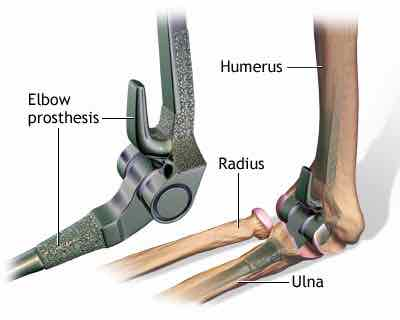
\includegraphics[scale=.5]{pics/prosthesis}
  \end{center}
  \item 消炎藥: anti-inflammatory
  \item 微創手術: minimally invasive surgery / key hole surgery
  \item 闌尾切除術: appendectomy (ectomy指...的手術)
  \item 心理準備: mentally prepared
  \item 主治醫生: attending doctor / attendings
  \item 大腿(根): thigh
  \item 血塊: blood clot
  \item 深靜脈血栓症: deep vein thrombosis
  \item 滑雪: skiing
  \item 私人醫生: private \hilight{health} insurance
  \item 自付費: out of pocket costs / expenses
  \item 最終決定: final say
\end{itemize}
\end{multicols}

\subsubsection*{需要掌握的句型}
\begin{itemize}
  \itemsep0em
  \item 做手術: perform the surgery / carry out the surgery
  \item 癱在床上: lie in bed paralysed
  \item 解釋怎麼做: explain how $sth.$ is done
  \item 新骨頭用什麼做的: What are the new bones made of?
  \item 關節磨損: wear and tear of joint (\hilight{worn表示磨損})
  \item 把...切除: have...removed
  \item 花...天恢復: It took me...days to recover.
  \item 請你注意: bear in mind
\end{itemize}

\subsection{哮喘發作}
\subsubsection*{需要掌握的單詞短語}
\begin{itemize}
  \itemsep0em
  \item 球場: pitch
  \item 上氣不接下氣: gasp for air
  \begin{center}
    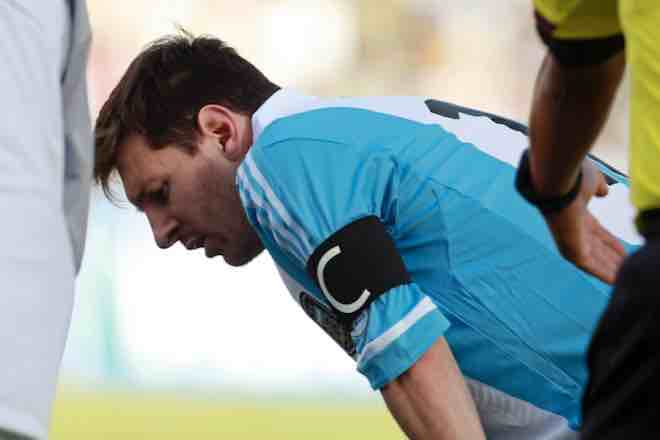
\includegraphics[scale=.3]{pics/gasp-for-air.jpg}
  \end{center}
  \item 預防性的藥物: preventative medications
  \item 支氣管擴張藥: bronchodilator agent (dilator指擴張劑)
  \item 對了, 說中了: Spot on!
  \item 四分之一決賽 / 半決賽 / 總決賽: quater-final /  semi-final / grand-final
  \item 我的疏忽: my own oversight
  \item (比賽的)隊長: captain
\end{itemize}

\subsubsection*{需要掌握的句型}
\begin{itemize}
  \itemsep0em
  \item 一開始慌神: I panicked at first.
  \item 謝謝關心: Thanks for caring.
  \item 突然, 無緣無故: out of the blue / out of sudden
  \item 你說對了: You got it spot on. / You hit the nail on the head!
  \item 不得不錯過: have to miss \hilight{out on}...
  \item 冒險去做: risk doing...
  \item 我還是...: I'd better...
\end{itemize}

\subsection{關節炎}
\subsubsection*{需要掌握的單詞短語}
\begin{itemize}
  \itemsep0em
  \item 風濕性 / 骨關節炎: rheumatic arthritis (維基百科查到rheumatoid arthritis) / osteoarthritis
  \item 老年病(專家): geriatric disease (geriatrics)
  \item 持續的疼: consistent pain, long-lasting pain
  \item 冰袋: icepack
  \item 減緩疼痛: kill / relieve / ease / alleviate the pain
  \item 遺傳缺陷: genetic predisposition
  \item 多補鈣: increase calcium intake
  \item 富含鈣: \hilight{rich} in calcium
  \item 耐力: endurance
\end{itemize}

\subsubsection*{需要掌握的句型}
\begin{itemize}
  \itemsep0em
  \item 在...大學讀書: study \hilight{at} ... university
  \item ...的原因是?: What are the causes of ...?
  \item (因為遺傳的)容易得某病: be predisposed to some disease
  \item 由...引起的: stem from...
  \item 當發作時吃止疼藥: take painkillers\footnote{服用painkiller的時候一般都是用複數} whenever it attacks / strikes / acts up
  \item 至於說...: as to...
  \item What should I pay attention to \hilight{in terms of} / \hilight{as to} my diet?
\end{itemize}

\subsection{高血壓}
\subsubsection*{需要掌握的單詞短語}
\begin{itemize}
  \itemsep0em
  \item 在晚年: in old age
  \item 遺傳性的疾病: genetic / hereditary / inherited disease
  \item 高膽固醇: high cholesterol
  \item 甲狀腺功能亢進症\footnote{甲狀腺功能活動過盛,甲狀腺激素分泌過多,其特徵是甲狀腺腫、心動過速或心房纖顫、脈壓增高、心悸、易疲勞、神\\經過敏和震顫、不耐熱、大量汗出、皮膚光滑濕熱、體重降低、肌肉虛弱、排便過多、情緒不穩以及眼部的症狀(如凝視、\\眼瞼遲滯、畏光,有時眼球突出)}: hyperthyroidism 
  \item 注意力不足過動症(多動症): Attention deficit hyperactivity disorder
  \item 重口味 / 輕口味食物: rich / plain flavour food
  \item 飲食習慣: eating habits
  \item 收縮壓 / 舒張壓: systolic / diastolic blood pressure (俗稱高低壓)
  \item 抗高血壓藥物: anti-hypertensive drugs
  \item 適量: in moderation
\end{itemize}

\subsection{肝炎}
\subsubsection*{需要掌握的單詞短語}
\begin{itemize}
  \itemsep0em
  \item 乙肝\footnote{又稱為血清性肝炎, 乙型病毒性肝炎, 是指乙肝病毒檢測為陽性, 病程超過半年或發病日期不明確而臨床有慢性肝炎表現者.} : hepatitis B
  \item 肝硬化: cirrhosis
  \item 感染病毒: catch the virus
  \item 餐具: eating utensils
  \item 接種: be vaccinated / get the vaccination
  \begin{center}
    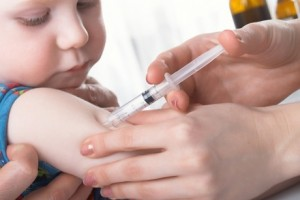
\includegraphics[scale=.7]{pics/vaccinated}
  \end{center}
\end{itemize}

\subsubsection*{需要掌握的句型}
\begin{itemize}
  \itemsep0em
  \item 電話里說...: tell $sth.$ \hilight{over} the phone
  \item 肝功能正常: Liver has been functioning properly.
  \item 和一般的驗血有區別嗎: Is it different to a general blood test?
\end{itemize}

\vspace{15mm}

\begin{center}
  \textbf{************ END OF THE DAY ************}
\end{center}

\newpage

\section{2016年2月9日 (Instructor: Chris)}
\mybox{\centering \textbf{注意}: 今天的更多內容請見詞彙專題里的Medicare詞彙!}
\subsection{皮膚癌}
\mybox{\centering \textbf{注意}: 本對話的更多內容請見詞彙專題里的``和皮膚病有關的詞"!}
\subsubsection*{需要掌握的單詞短語}
\begin{multicols}{3}
\begin{itemize}
  \itemsep0em
  \item 發生率: incidence
  \item 發病率: morbidity
  \item 死亡率: mortality
  \item 紫外線: UV rays
  \item 臭氧層: ozone layer
  \begin{center}
    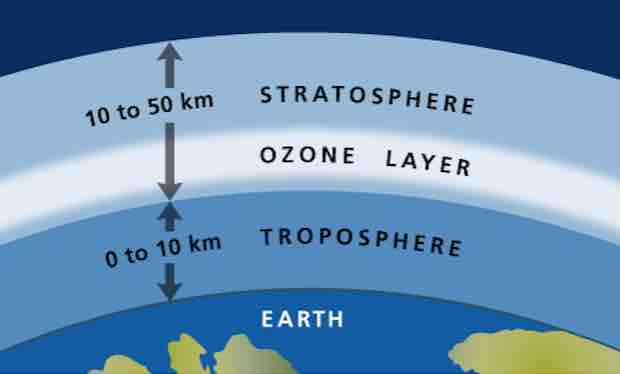
\includegraphics[scale=.25]{pics/ozone-layer}
  \end{center}
  \item 陽傘: parasol
  \item 防曬霜: sunscreen
  \item 防曬指數: Sun Protect Factor (SPF)
  \item 可防曬的衣服: protective clothing
  \item 太陽鏡: sunglasses (sunnies)
  \item 自由基\footnote{自由基, 係氧在體內新陳代謝後所產生的物質, 它的活性極強, 可與任何物質發生強烈的反應.}: free radical (加速皮膚老化)
  \item 活檢: biopsy\footnote{活體組織切片檢查}
  \item 中暑: sunstroke
  \item 曬傷: sunburn
  \begin{center}
    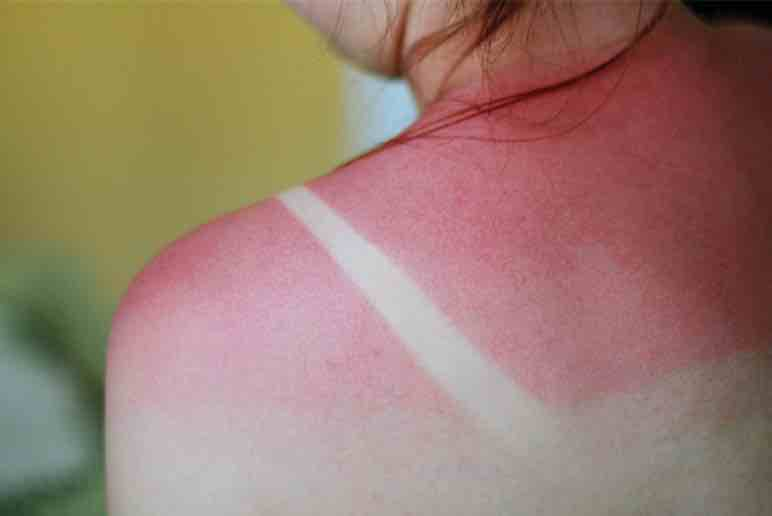
\includegraphics[scale=.2]{pics/sunburn}
  \end{center}
  \item outdoor = in the open air
  \item 暴露, \hilight{接觸}(輻射) = exposure
  \item 充足的防護: adequate protection
  \item 塗(防曬霜): apply
  \item 藥膏: cream ointment
  \item cure $vs.$ treat: 治癒 $vs.$ 治療
  \item 減少, 淘汰: eliminate
  \item 豬流感: \hilight{swine} flu
  \item 禽流感: \hilight{bird} flu
\end{itemize}
\end{multicols}

\subsubsection*{需要掌握的句型}
\begin{itemize}
  \itemsep0em
  \item 在我的手臂上: on my arm
\end{itemize}

\subsection{水痘 (共兩部分)}
\subsubsection*{需要掌握的單詞短語}
\begin{multicols}{2}
\begin{itemize}
  \itemsep0em
  \item body = trunk
  \item 低燒: mild fever
  \item 學徒: trainee
  \item 病毒性疾病: viral disease
  \item 火(爆)了: go viral
  \item 扇耳光: slap \hilight{in} face
  \item 肺炎 / 腦炎\footnote{腦炎是指腦實質受病原體侵襲導致的炎症性病變.}: pneumonia / encephalitis
  \item 爐甘石洗液: calamine lotion
  \begin{center}
    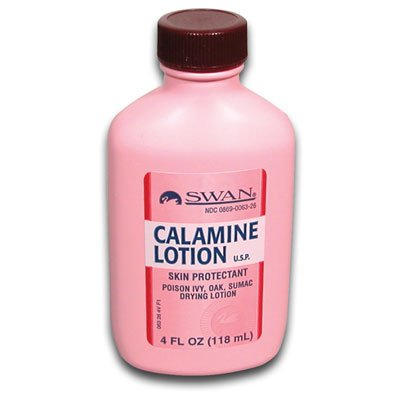
\includegraphics[scale=.4]{pics/calamine-lotion}
  \end{center}
  \item 褥瘡: bedsore
  \begin{center}
    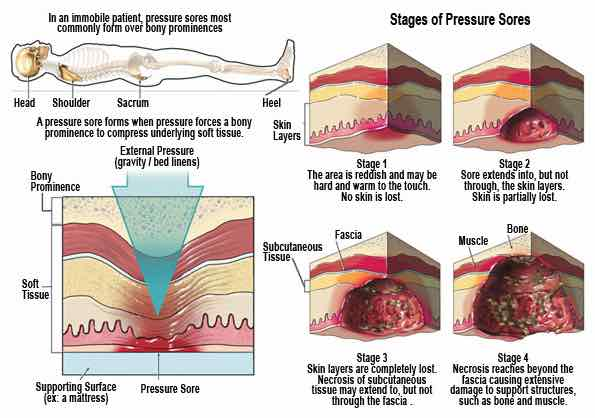
\includegraphics[scale=.4]{pics/bedsore}
  \end{center}
  \item 麻醉藥膏: anaesthetic cream
  \item 溫水 / 熱水 / 開水: \hilight{lukewarm} / warm / hot water
\end{itemize}
\end{multicols}

\subsubsection*{需要掌握的句型}
\begin{multicols}{2}
\begin{itemize}
  \itemsep0em
  \item 有一點發燒: A bit of temperature
  \item 我現在想起來: \hilight{Now that I come to think of it.}
  \item 與...相一致: be \hilight{consistent} with...
  \item 一定是被傳染: must have \hilight{contracted} / got / caught
  \item Chances are...: (放句首) 很有可能...
  \item ``一定一定": Most definitely / absolutely!
  \item 非常非常忙於: be overwhelmed by...
  \item 這也太煩了: What a nuisance! (nuisance單指心煩的事情)
  \item 生殖部位潰瘍: Sores in the \hilight{genital} area.
\end{itemize}
\end{multicols}

\subsection{丈夫不愛我了}
\subsubsection*{需要掌握的單詞短語}
\begin{itemize}
  \itemsep0em
  \item 讓我瘋了: drive me nuts / crazy
  \item 非常不開心, 感到痛苦的: distressing
  \item 出軌 / 出櫃: have an affair / come out of closet
  \item 各種家庭暴力的方式:
  \begin{enumerate}
    \itemsep0em
    \item 冷暴力: cold violence
    \item 情感上的折磨: emotional abuse
    \item 經濟上的\hilight{掌控}: financial abuse (在澳洲算家庭暴力)
    \item 言語辱罵: verbal abuse
    \begin{center}
      
\includegraphics[scale=.5]{pics/abuse}
      
\includegraphics[scale=.3]{pics/verbal-abuse}
    \end{center}
  \end{enumerate}
  \item 打(人): hit, beat, bash(狂揍)
  \item 揍了我一頓: beat me up
  \item 疏忽: oversight, negligence
\end{itemize}

\subsubsection*{需要掌握的句型}
\begin{multicols}{2}
\begin{itemize}
  \itemsep0em
  \item 這是一個友好的提醒: This is a \hilight{friendly / gentle} reminder that...
  \item 無計可施, 束手無策:
  \begin{enumerate}
    \itemsep0em
    \item My hands are tied.
    \item I have no options.
    \item I have no way out.
  \end{enumerate}
  \item 大束玫瑰: A big bunches of roses.
  \item 最近才...: It is \hilight{only} recently that...
  \item 主動提出: offer to do...
  \item 值得一試: worth a try / shot / go
\end{itemize}
\end{multicols}

\subsubsection*{注意}
\begin{itemize}
  \item ``When he back home" 是錯誤的用法, 應該改成``When he comes back home".
\end{itemize}

\subsection{精神分裂}
\subsubsection*{需要掌握的單詞短語}
\begin{multicols}{2}
\begin{itemize}
  \itemsep0em
  \item 罵人: swear / yell \hilight{at} $sb.$
  \item 精神崩潰: mental breakdown
  \item 誓言: vow
  \item 睡得很死: deep sleep
  \item 認為(正式): perceive (perception 表示感知)
  \item 正經的, 得體的: decent $\xrightarrow{\text{反義}}$ indecent (骯臟的)
  \item 同齡人: peers / people of his age
  \item 不睡覺: stay up (翻成``熬夜"即可)
  \item 問題男孩: difficult boy (難相處, 事情多, 老惹麻煩)
\end{itemize}
\end{multicols}

\subsubsection*{需要掌握的句型}
\begin{itemize}
  \itemsep0em
  \item 腦子不好使: \hilight{I can't think things clearly. / I can't think straight.}
  \item 累垮: \hilight{wear $sb.$ out.}
  \item 崩潰的邊緣: on the verge / edge of breakdown / collapse
  \item 他生病是因為...: He is sick in the sense that...
  \item 像我們這樣的正經家庭: decent family like ours
\end{itemize}

\subsubsection*{注意}
\begin{multicols}{2}
\begin{itemize}
  \itemsep0em
  \item lie / lied / lied 說謊
  \item lie / lay / lain 位於,躺
  \item lay / laid / laid: 置放, 鋪, 產 (蛋, 卵)
\end{itemize}
\end{multicols}

\subsection{疑似抑鬱的男孩}
\subsubsection*{需要掌握的單詞短語}
\begin{multicols}{2}
\begin{itemize}
  \itemsep0em
  \item 不情願: unwilling / reluctant ($adj.$)
  \item 小題大做: over-concerned
  \item 情緒低落: feel down
  \item 罪魁禍首: culprit
  \item 自卑: unconfident / self-abased
  \item 侮辱 / 羞辱: insult / humiliate
  \item 蔑視 / 嘲笑: contempt / tease
  \item 自殺傾向: suicidal tendency
  \item 遵守法律: observe the law
  \item 不開心的: low / down / gloomy / blue
\end{itemize}
\end{multicols}

\subsubsection*{需要掌握的句型}
\begin{multicols}{2}
\begin{itemize}
  \itemsep0em
  \item 他更不情願來了: He was more reluctant to come.
  \item 讓某人思想負擔過重: overburden of someone's mind.
  \item 看不起: look down upon...
  \item 假想出來的畫面: image from your assumption
  \item 被...發現: got caught by...
  \item 偶爾: once in a while
  \item 做某事是有道理的: have points in doing $sth.$
\end{itemize}
\end{multicols}

\vspace{15mm}

\begin{center}
  \textbf{************ END OF THE DAY ************}
\end{center}